\documentclass[12pt]{article}
\usepackage[utf8]{inputenc}
\usepackage{amsmath}
\usepackage{amsfonts}
\usepackage{amssymb}
\usepackage{hyperref}
\usepackage[a4paper, total={6in, 8in}]{geometry}
\usepackage{graphicx}
\usepackage{xcolor}
\usepackage{tcolorbox}
\usepackage{tikz}
\usetikzlibrary{arrows,automata}
\usepackage{pgf}


\definecolor{mytransparentcolor}{rgb}{0.8,0.2,0.3} % Beispiel RGB-Farbe

\title{N-gram Language Models}
\author{
  Felix Pötzsch\\
  \and
  Borisov Timofei \\
  \and
  Simon \\
}
\date{\today}

\begin{document}

% Title page
\maketitle

% Abstract
\begin{abstract}
	This is a brief summary of your essay. It should be concise and informative.
\end{abstract}

% Table of contents
\tableofcontents
\clearpage

% Sections
\section{Introduction}

\subsection{Sprachmodelle}
Sprachmodelle sind der Versuch beispielsweise natürliche Sprache als mathematisches 
Modell darstellen zu können. Ihnen liegt meist ein stochastischer Prozess zugrunde. 
Bekannte Modelle sind:

\begin{itemize}
	\item RNN (Rekurrente Neuronale Netze)
	\begin{itemize}
        \item[-] Abhängigkeiten zwischen Wörtern können erfasst werden und so kontextuell, kohärente Sätze gebildet werden.
        \item[-] Verschwindender Gradient. Abhängigkeiten in großer Entfernung können nicht mehr erkannt werden.
    \end{itemize}
	\item LSTM (Long Short-Term Memory)
	\begin{itemize}
        \item[-] Art von RNN die das Problem des verschwindenden Gradienten durch Speicherzellen lösen.
        \item[-] Zelle ermöglicht selektives merken oder vergessen, wodurch langfristige Abhängigkeiten berücksichtigt werden können.
    \end{itemize}
	\item GRU:
	\begin{itemize}
        \item[-] Zielen darauf ab, die Architektur von LSTMs zu vereinfachen und gleichzeitig das Problem des verschwindenden Gradienten anzugehen.
        \item[-] Weniger Gating- Mechanismen aber dafür Rechenintensiver.
        \item[-] Haben eine vergleichbare Leistung wie LSTM.
    \end{itemize}
	\item Transformer Modelle:
	\begin{itemize}
		\item[-] GPT
		\begin{itemize}
			\item[-] Im Gegensatz zu RNN benutzen Transformer Selbstaufmerksamkeitsmechanismen.
			\item[-] Transformatoren verarbeiten Wörter parallel, was zu höherer Effizienz führt.
		\end{itemize}
        \item[-] GPT4
		\begin{itemize}
			\item[-] Ist im Gegensatz zu GPT3 (1,76 Billionen Parameter) kein monolithisches Sprachmodell mehr sondern eher eine Mischung aus 8 x 220 Milliarden Parametermodellen. 
			\item[-] Umfangreicher Textkorpus.
			\item[-] Besonders gut für kohärente und kontextrelevante Texte.
			\item[-] Kann für Vielzahl von Anwendungen verwendet werden, z.B.: Code-generierung. 
		\end{itemize}
    \end{itemize}
\end{itemize}


Im Voraus sollten bei diesen Modellen sowohl Kenntnisse über Sprache im Allgemeinen bestehen, sowie über die jeweilige Kommunikationssituation. Die oben genannten Modelle bestehen zudem aus mehreren Teilmodellen. Meist sind das Vokabular, Häufigkeiten und Grammatik. Die oben genannten Modelle treten zudem in Kombination auf.
Sprachmodelle lassen sich in 4 verschiedene Sorten einteilen: 

\begin{itemize}
	\item Regelbasierte Systeme
	\begin{itemize}
		\item[-] Vordefinierte Sprachregeln, Vorlagen.
		\item[-] Fehlende Fähigkeit kontextrelevante dynamische Text zu generieren.
	\end{itemize}
	\item Vorlagenbasierte Systeme
	\begin{itemize}
		\item[-] Vordefinierte Vorlagen, die mit dynamischen Inhalten gefüllt werden.
		\item[-] Gewisses Maß an Anpassung möglich (Grammatik).
		\item[-] Kein einzigartiger kreativer Text. 
	\end{itemize}
	\item Statistische Sprachmodelle
	\begin{itemize}
		\item[-] N-Gramme, Markov (HMM)
		\item[-] Mangel an semantischem Verständnis und Schwierigkeiten kontextrelevante Inhalte zu erzeugen.
	\end{itemize}
	\item Neuronale Sprachmodelle
	\begin{itemize}
		\item[-] Dialoge sind möglich und es können sowohl Kontextrelevante als auch Kohärente Teile erkannt werden.
		\item[-] Siehe RNN, LSTM, GRU, GPT 
	\end{itemize}
\end{itemize}

\subsection{N-Gramme}
N-Gramme, sind in der Linguistik eine Sequenz von N aufeinanderfolgenden Fragmenten eines Textes. Fragmente können dabei Buchstaben, Silben, Laute oder Wörter sein. Das können von 1-Gramm (Uni-Gramme), über 2-Gramm (Bi-Gramme), 3-Gramm (Tri-Gramme) bis Multigrammen sein. Ihnen zugrunde liegt die Markov-Annahme. Die Markov-Annahme erschließt eine Vorhersage über einen zukünftigen Zustand nicht aus der Menge aller Zustände, sondern nur der unmittelbaren vorherigen eingetretenen Zustände. Die Zustände können in diesem Falle als Fragmente aufgefasst werden. Die klassischen Anwendungsgebiete für N-Gramme liegen in der Rechtschreibkorrektur, Textvervollständigung/Wörter vorhersage (z.B.: SMS schreiben), Textanalyse (Beurteilung), Spracherkennung (Audioanwendungen) und Handschrifterkennung.\\

\noindent \textbf{Typische N-Gramme:}
\\
\\
\\
Unigramm:
\\
$N = 1$: 	\fbox{\raisebox{0pt}[0.3cm][0.05cm]{\strut This}}
			\fbox{\raisebox{0pt}[0.4cm][0.15cm]{\strut is}} 
			\fbox{\raisebox{0pt}[0.5cm][0.25cm]{\strut a}} 
			\fbox{\raisebox{0pt}[0.6cm][0.35cm]{\strut sentence}}.
			\begin{tikzpicture}[baseline={(current bounding box.center)}]
				\coordinate (A) at (0,0.4);
				\coordinate (B) at (3,1);
				\coordinate (C) at (0,-0.2);
				\coordinate (D) at (3,-1);
				\draw (A) -- (B);
				\draw (C) -- (D);
			\end{tikzpicture}
			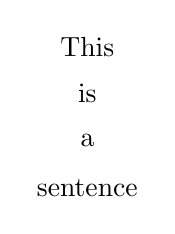
\begin{tikzpicture}[baseline={(current bounding box.center)}]
				\node at (2,0.9) {This};
				\node at (2,0.3) {is};
				\node at (2,-0.3) {a};
				\node at (2,-0.9) {sentence};
			\end{tikzpicture}
\\
\\
\\
Bigramm:
\\
$N = 2$: 	\fbox{\raisebox{0pt}[0.3cm][0.05cm]{\strut This is}}
			\hspace{-0.6cm}\fbox{\hspace{0.4cm}\raisebox{0pt}[0.4cm][0.15cm]{\strut a}} 
			\hspace{-0.6cm}\fbox{\hspace{0.4cm}\raisebox{0pt}[0.5cm][0.25cm]{\strut sentence}}.
			\begin{tikzpicture}[baseline={(current bounding box.center)}]
				\coordinate (A) at (0,0.4);
				\coordinate (B) at (3,1);
				\coordinate (C) at (0,-0.2);
				\coordinate (D) at (3,-1);
				\draw (A) -- (B);
				\draw (C) -- (D);
			\end{tikzpicture}
			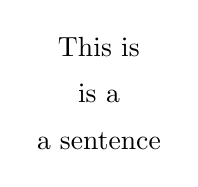
\begin{tikzpicture}[baseline={(current bounding box.center)}]
				\node at (2,0.9) {This is};
				\node at (2,0.3) {is a};
				\node at (2,-0.3) {a sentence};
			\end{tikzpicture}
\\
\\
\\
Trigramm:
\\
$N = 2$: 	\fbox{\raisebox{0pt}[0.3cm][0.05cm]{\strut This is a}}
			\hspace{-0.6cm}\fbox{\hspace{0.4cm}\raisebox{0pt}[0.4cm][0.15cm]{\strut sentence}}.
			\begin{tikzpicture}[baseline={(current bounding box.center)}]
				\coordinate (A) at (0,0.4);
				\coordinate (B) at (3,1);
				\coordinate (C) at (0,-0.2);
				\coordinate (D) at (3,-1);
				\draw (A) -- (B);
				\draw (C) -- (D);
			\end{tikzpicture}
			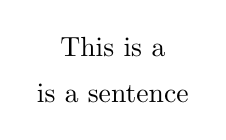
\begin{tikzpicture}[baseline={(current bounding box.center)}]
				\node at (2,0.9) {This is a};
				\node at (2,0.3) {is a sentence};
			\end{tikzpicture}
\clearpage

\noindent Die daraus folgende typische Markov Annahme als Prozessdiagramm und Übergangstabelle:
\\
\\
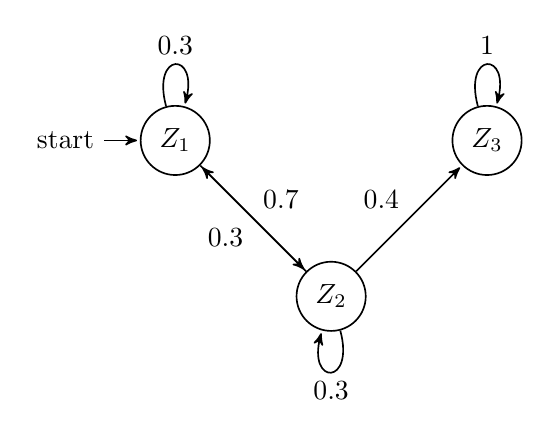
\begin{tikzpicture}[->,>=stealth',shorten >=1pt,auto,node distance=2.8cm, semithick]
	
	\tikzstyle{every state}=[fill=white,draw=black,text=black]

	\node[initial,state] (A)                    {$Z_1$};
	\node[state]         (B) [below right of=A] {$Z_2$};
	\node[state]         (C) [above right of=B] {$Z_3$};

	\path 	(A) edge [loop above] node {0.3} (A)
			(B) edge node {0.3} (A)
			(A) edge node {0.7} (B)
			(B) edge [loop below] node {0.3}
			(B)	edge              node {0.4} (C)
			(C) edge [loop above] node {1} (C);

\end{tikzpicture}
\\
\\
Grundsätzlich haben wir es mit einer Bedingten Wahrscheinlichkeit zu tun die wie folgend aussieht:

\begin{equation}
	\begin{split}
	P(t) = P(w_1, w_2,...w_n) &= P(w_1)*P(w_2 \mid w_1)...P(w_n \mid w_1,...w_n-1) \\ 
	&= \prod_{i=1}^{n} P(w_i \mid w_1...w_i-1)
	\end{split}
\end{equation}

\begin{equation}
	P(w_1 \mid w_1...w_i-1) = \frac {P(w_1...w_i)}{P(w_1...w_i-1)}
\end{equation}
\\
Also die Wahrscheinlichkeit das Wort 1 eintritt unter der Bedingung, dass ein Paar andere Wörter vorher 
schon in Kombination aufgetreten sind. Demnach wird Text auf Basis von statistischen Mustern generiert 
oder anders gesagt: Neu angeordnet. Es mangelt dadurch häufig an semantischem Verständnis. Insbesondere 
im Zusammenhang mit langfristigeren Abhängigkeiten (Kohärenz) sind Sprachmodelle die rein auf N-Grammen 
basieren sehr ungeeignet, um Texte zu schreiben. Da lediglich auf Basis einer \textit{Maximum-Likelyhood} Methode 
gearbeitet wird, kann Text nur \textit{nacherzählt} werden aber nicht generiert.\\
Es folgen nun ein paar typischen Eigenheiten von N-Grammen. Einem Totalversagen entgegenzuwirken, muss 
zunächst die Wahl eines geeigneten N priorisiert werden. Denn auch wenn ein geeigneter (Text-) Korpus 
gut gewählt wurde kann es zu \textit{Unseen N-Grams} kommen. Ebenso wie \textit{Unseen N-Grams} gibt es 
auch \textit{Unseen/Unknown Words}. Prinzipiell aber sollte gesagt werden, dass auch ein großer oder geeigneter Korpus nicht immer zum 
Erfolg führt, da auch dort Wortkombinationen oder Wörter \textit{Unseen} sein können (Chomsky, Zipfsches Gesetz). 
Des Weiteren sollte auf den Underflow bei der Bewertung der Wahrscheinlichkeiten geachtet werden. Dieses 
Problem führt zum nächsten, denn es müssen nicht nur zu niedrige, sondern auch die vollständigen 
Nullwahrscheinlichkeiten beachtet werden.\\
Es müssen also vor allem die Informationen in Form der Angepasstheit sowie Auswahl vorab gut gewählt werden 
sowie die im Folgenden beschrieben Techniken des \textit{Smoothings}, also der Re-evaluation von 
Nullwahrscheinlichkeiten und niedrigen Wahrscheinlichkeiten eigesetzt werden. Dazu zählt ebenfalls die 
zusätzlich im Folgenden beschriebene Perplexität als Evaluationstechnik, um auf \textit{Back Off Words}, also 
Wörter, auf welche ausgewichen werden kann, zu kommen.

\clearpage
\section{Fortgeschrittene Konzepte und Techniken in N-Gramm-Modellen (Borisov Timofei)}
\subsection{Was ist un-seen N-Grams?}
Da jeder Corpus begrenzt ist, fehlen darin zwangsläufig einige völlig akzeptable Wortfolgen. Das heißt, wir werden viele Fälle von vermeintlichen "zero probability n-grams" haben, die in Wirklichkeit eine Nicht-Null-Wahrscheinlichkeit haben sollten \cite{jurafsky2023}.

Betrachten wir die Wörter, die auf das Bigram aus Daniel Jurafskys Buch basieren. Ein Textkorpus zusammen mit ihrer Anzahl:

\begin{itemize}
	\item denied the allegations: 5
	\item denied the speculation: 2
	\item denied the rumors: 1
	\item denied the report: 1
\end{itemize}

Aber nehmen wir an, unser Testsatz enthält Sätze wie:
\begin{itemize}
	\item denied the offer
	\item denied the loan
\end{itemize}

P(offer|denied the) ist 0!
P(loan|denied the) ist 0!

Diese Nullen bedeuten, dass wir die Wahrscheinlichkeit anderer Wortkombinationen stark unterschätzt haben, was die richtige Entscheidung der Anwendung, die auf unserem Modell läuft, stark beeinflussen könnte.

Das Problem heißt “Data Sparsity” \cite{dremio2023}. Also kurz gesagt, das bedeutet, dass viele Daten in einem Datensatz fehlen oder auf Null gesetzt sind, sodass die meisten Zellen in einer Tabelle leer bleiben. Dies tritt häufig bei spärlichen Matrizen oder hochdimensionalen Datensätzen auf, wo nicht alle Elemente beobachtet oder erfasst werden. Was können wir also mit den Wörtern machen, die wir verwenden und die nicht in den Kontext unserer Trainingsdaten passen?

Die Methode zur Lösung dieses Problems heißt: Smoothing oder Discounting.

\subsection{Smoothing Techniques}
\subsubsection{Laplace-Glättung. Add One (Add X).}
Die einfachste Art der Glättung besteht darin, zu allen n-Gramm-Zählungen einen Wert zu addieren, bevor wir sie zu Wahrscheinlichkeiten normalisieren. Alle Zählungen, die vorher Null waren, haben nun den Wert 1, die Zählungen von 1 werden zu 2 usw. Dieser Algorithmus wird als Laplace-Glättung oder Additive Glätterung bezeichnet \cite{foster2020}.

Statt
\begin{center}
	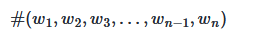
\includegraphics[width=0.3\textwidth]{statics/Borisov/1.PNG}
\end{center}

Wir setzen
\begin{center}
	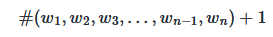
\includegraphics[width=0.4\textwidth]{statics/Borisov/2.PNG}
\end{center}

Da das Vokabular aus V-Wörtern besteht und jedes Wort inkrementiert wurde, müssen wir auch den Nenner anpassen, um die zusätzlichen V-Beschachtungen zu berücksichtigen.
\begin{center}
	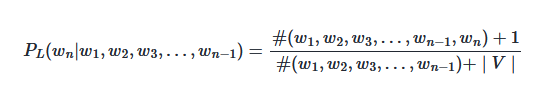
\includegraphics[width=0.6\textwidth]{statics/Borisov/3.PNG}
\end{center}

\cite{maucher2022}

Eine Alternative zur Glättung durch Addition besteht darin, einen etwas geringeren Anteil der Wahrscheinlichkeitsmasse von den gesehenen zu den ungesehenen Ereignissen zu verschieben. Anstatt zu jeder Zählung 1 zu addieren, fügen wir einen Bruchteil der Zählung k hinzu.
\begin{center}
	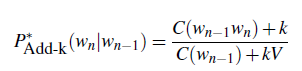
\includegraphics[width=0.4\textwidth]{statics/Borisov/4.PNG}
\end{center}

\cite{jurafsky2023}.

\subsubsection{Good-Turing Glättung}
Wie berechne ich die Wahrscheinlichkeit von un-seen N-Grams?

Der erste Schritt der Berechnung besteht darin, die Wahrscheinlichkeit abzuschätzen, dass ein zukünftig beobachtetes Fall zu einer bisher nicht gesehenen Art gehört. Diese Schätzung ist:
\begin{center}
	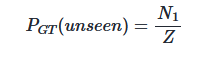
\includegraphics[width=0.3\textwidth]{statics/Borisov/5.PNG}
\end{center}

Der nächste Schritt besteht darin, die Wahrscheinlichkeit zu schätzen, dass das nächste beobachtete Fall einer Art angehört, die bereits r-mal beobachtet wurde. Für eine einzelne Art beträgt diese Schätzung:
\begin{center}
	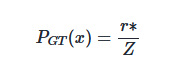
\includegraphics[width=0.2\textwidth]{statics/Borisov/6.PNG}
\end{center}
Good-Turing-Smoothing löst dieses Dilemma, indem es die Häufigkeitswerte anpasst. Es wird so getan, als ob Arten, die eigentlich r-mal vorkommen, \( r^* \)-mal vorkommen, mit
\begin{center}
	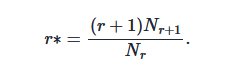
\includegraphics[width=0.3\textwidth]{statics/Borisov/7.PNG}
\end{center}
\cite{maucher2022}, \cite{gale1995}

\subsubsection{Katz Backoff Glättung}
\quad Wenn ein benötigtes n-Gramm in einem Backoff-N-Gramm-Modell keine Vorkommen aufweist, gehen wir zum (n-1)-Gramm über. Dieser Prozess wird fortgesetzt, bis wir eine Sequenz finden, die einige Vorkommen hat.
\\ Damit ein Backoff-Modell eine korrekte Wahrscheinlichkeitsverteilung ergibt, müssen die n-Gramme höherer Ordnung reduziert werden, um etwas Wahrscheinlichkeitsmasse für die n-Gramme niedrigerer Ordnung zu reservieren. Ähnlich wie bei der Add-One-Glättung führt die Verwendung der nicht diskontierten MLE-Wahrscheinlichkeit dazu, dass bei der Ersetzung eines n-Gramms mit einer Wahrscheinlichkeit von Null durch ein n-Gramm niedrigerer Ordnung zusätzliche Wahrscheinlichkeitsmasse hinzugefügt wird. Dies würde dazu führen, dass die Gesamtwahrscheinlichkeit, die das Sprachmodell allen möglichen Zeichenketten zuweist, größer als 1 ist. Neben diesem expliziten Abzinsungsfaktor benötigen wir eine Funktion a, um diese Wahrscheinlichkeitsmasse auf die n-Gramme niedrigerer Ordnung zu verteilen.
\\ \\Beim Katz-Backoff stützen wir uns auf eine diskontierte Wahrscheinlichkeit P*, wobei wir rekursiv auf die Katz-Wahrscheinlichkeit für das (n-1)-Gramm mit kürzerer Vorgeschichte zurückgehen. Die Wahrscheinlichkeit für ein Backoff n-Gramm PBO wird also wie folgt berechnet:
\begin{center}
	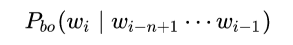
\includegraphics[width=0.4\textwidth]{statics/Borisov/8.PNG}
\end{center}
\begin{center}
	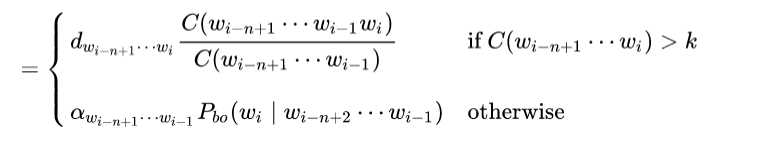
\includegraphics[width=0.7\textwidth]{statics/Borisov/9.PNG}
\end{center}

\quad Zur Berechnung von $\alpha$ ist es sinnvoll, zunächst eine Größe $\beta$ zu definieren, die die verbleibende Wahrscheinlichkeitsmasse für das $(n - 1)$-Gramm darstellt:


\begin{center}
	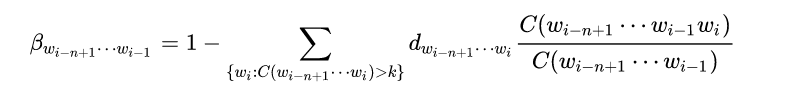
\includegraphics[width=0.8\textwidth]{statics/Borisov/10.PNG}
\end{center}

Anschließend:

\begin{center}
	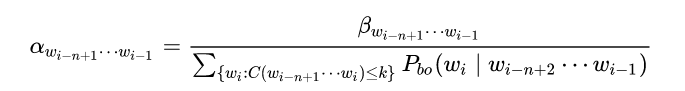
\includegraphics[width=0.8\textwidth]{statics/Borisov/11.PNG}
\end{center}

\subsection{Vergleich von N-Grammen und neuronalen Netzen.}
\quad Im Allgemeinen sind neuronale Netze fortschrittlichere und komplexere Instrumente als N-Gramme. Ihr Vorteil liegt in vielen Aspekten. Zum Bespie: N-Gramme erfassen nur den lokalen Kontext. Ein Trigramm-Modell berücksichtigt nur zwei vorangehende Wörter, um das nächste Wort vorherzusagen. Sie sind nicht in der Lage, weitreichende Abhängigkeiten zu verstehen. Mit steigendem Wert von "n" wächst die Zahl der möglichen n-Gramme exponentiell, was zu hohem Speicherverbrauch und Sparsamkeitsproblemen führt. Probleme mit Wörtern, die mehrere Bedeutungen haben (Polysemie), oder mit verschiedenen Wörtern, die gleich klingen (Homonymie), weil ihnen ein tiefes Verständnis des Kontextes fehlt. N-Grams erfordern manuelles Feature-Engineering, um die relevanten n-Gramme auszuwählen, und führen oft zu hochdimensionalen, spärlichen Vektoren usw.

\cite{roshmita2023}
\cite{clarkGiorgoloLappin}
\\
Neuronale Netze sind mittlerweile kontextbewusst. Insbesondere mit Architekturen wie LSTM (Long Short-Term Memory) oder Transformer-Modellen können neuronale Netze weitreichende Abhängigkeiten und kontextuelle Informationen über ganze Sätze oder sogar Absätze hinweg erfassen. Sie verfügen über ein automatisches Lernen von Merkmalen während des Trainingsprozesses, wodurch sich der Bedarf an umfangreicher manueller Merkmalstechnik verringert usw.Wir müssen jedoch den Vorteil von N-Grammen anerkennen. Bei kurzen Texten sind N-Gramm-Methoden dem neuronalen Netz überlegen.
\cite{babukumar2010}

\section{Main Section 3 (SIMON)}
\subsection{Subsection 3.1}
Discuss the details of your third main point.
\subsection{Subsection 3.2}
Further details and analysis related to your third main point.

\section{Conclusion}
Summarize the main points discussed in your essay and provide your final thoughts.

% Bibliography
\clearpage
\begin{thebibliography}{9}

	\bibitem{jurafsky2023}
	Daniel Jurafsky and James H. Martin, \textit{Speech and Language Processing}, 3rd Edition, Pearson, 2023.

	\bibitem{dremio2023}
	Dremio, ``Data Sparsity,'' \url{https://www.dremio.com/wiki/data-sparsity/}, Accessed: June 1, 2024.

	\bibitem{foster2020}
	David Foster, \textit{Generative Deep Learning: Teaching Machines to Paint, Write, Compose, and Play}, O'Reilly Media, 2020.

	\bibitem{maucher2022}
	Prof. Dr. Johannes Maucher \url{https://griesshaber.pages.mi.hdm-stuttgart.de/nlp/04ngram/01ngram.html}, Accessed: June 1, 2024.

	\bibitem{gale1995}
	William A. Gale, "Good–Turing smoothing without tears," \textit{Journal of Quantitative Linguistics}, 1995.

	\bibitem{roshmita2023}
	Roshmita Dey , Accessed: June 1,\textit{Understanding Language Modeling: From N-grams to Transformer-based Neural Models} 2024.

	\bibitem{clarkGiorgoloLappin}
	Alexander Clark, Gianluca Giorgolo, and Shalom Lappin, \textit{Statistical Representation of Grammaticality Judgements: the Limits of
		N-Gram Models}, Department of Philosophy, King’s College London

	\bibitem{babukumar2010}
	A. Suresh Babu, Kumar P.N.V.S.Pavan
	\textit{Comparing Neural Network Approach with N-Gram Approach for Text Categorization},     January 2010International Journal on Computer Science and Engineering 2(1)

\end{thebibliography}

\end{document}
